% !TEX root = DesignDocument.tex

\section{Mobile Testing}
    Testing for the mobile app was primarily done manually. This is because most testing was done on visualizing files and verifying the app performed as expected.  It was also verifying that HTTP packets were as expected going to and from the phone.

    \subsection{Files}
        A variety of files were used throughout development to test functionality of the app. Some sample files were found on \url{https://free3d.com}. Some files were provided from Dr. Deschamp and others were generated in Maple. Different files were used to test that colors were working both in the MTL and as PNGs. Additionally, large and small files were tested to see how the app reacted to more complex files. The BMW file seen below is an example of a complex file that didn't render well in our app that shows the limitations of our app.
        
        \subsubsection{Colors}
        
            A major feature requested for the app was to be able to display colors. The example below shows a simple sphere with a proof of concept that colors do work. The car is a more in-depth example that shows multiple colors on the same model.
            
            \begin{figure}[H]
                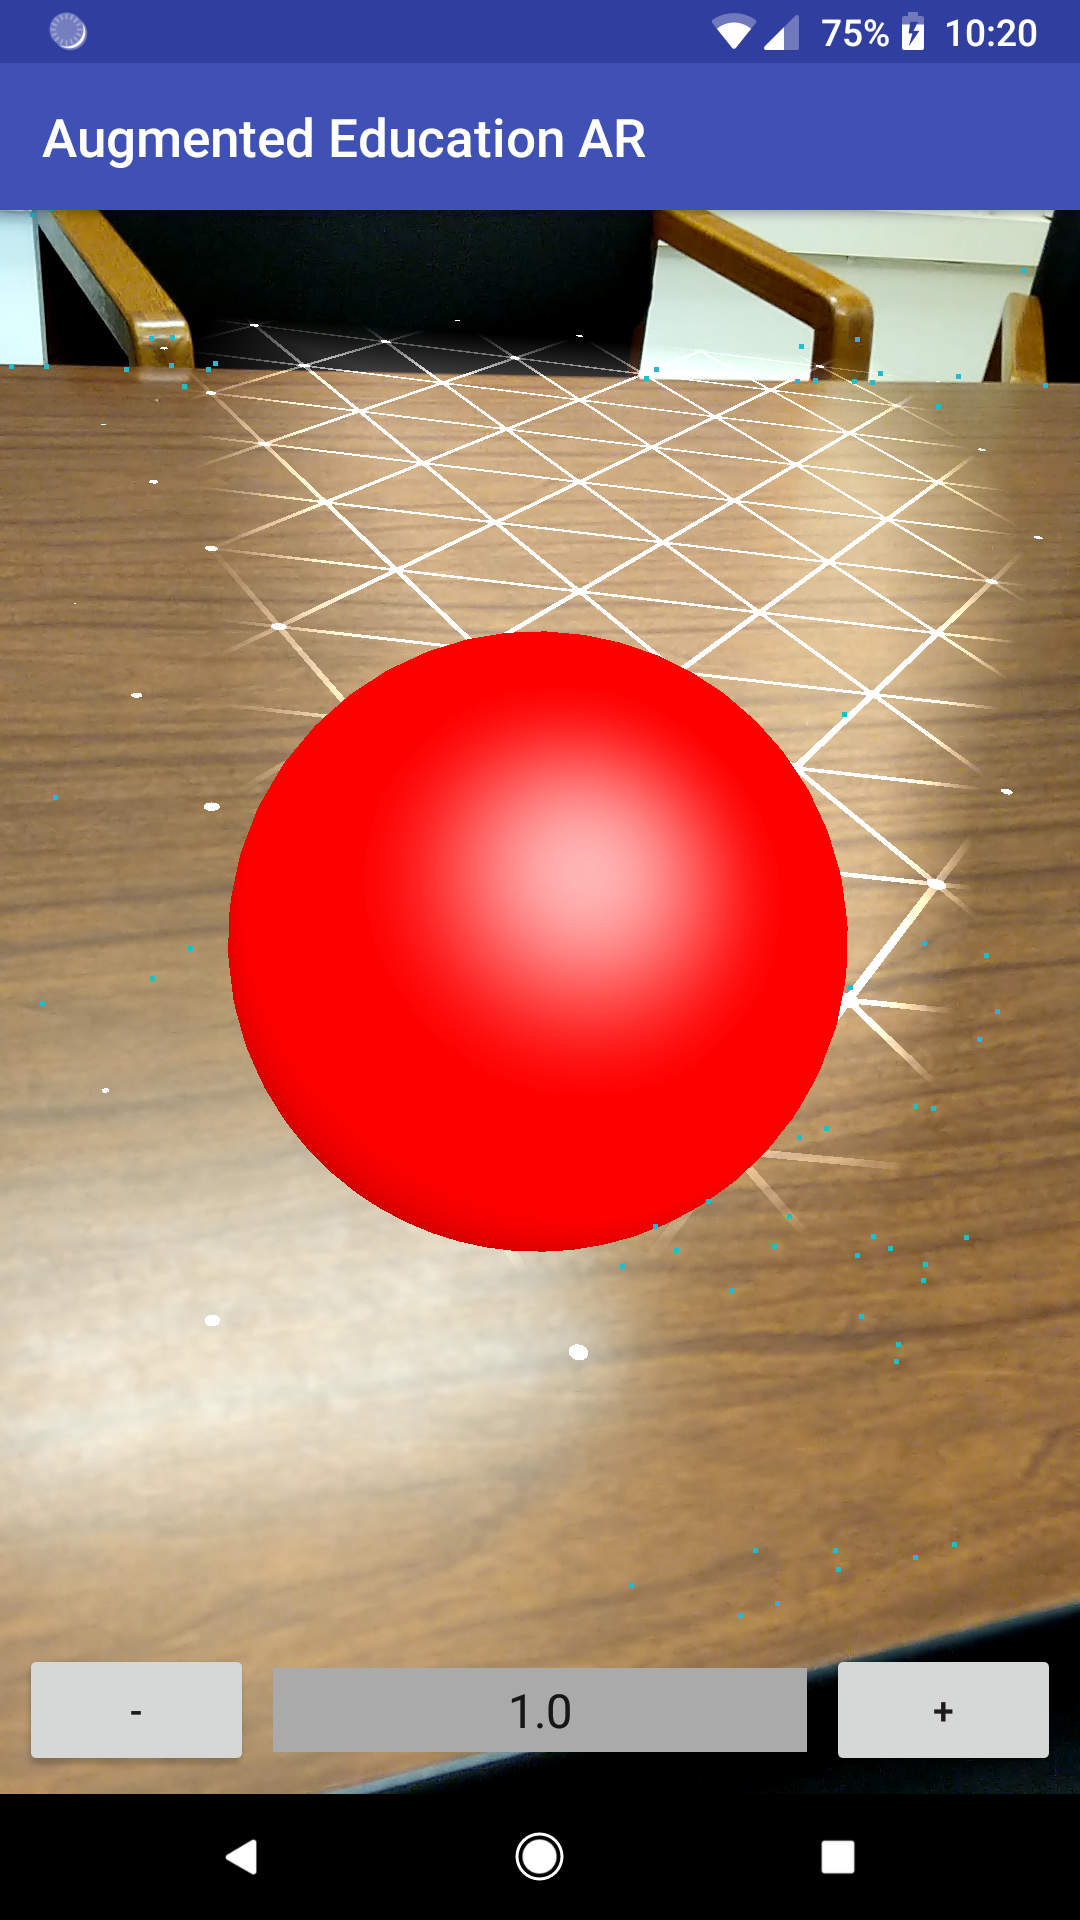
\includegraphics[width=0.5\textwidth]{Mobile/Mobile_RedSphere}
                \centering
                \caption{Colors - Red Sphere}
                \label{fig:mobileRedSphere}
            \end{figure}

            \begin{figure}[H]
                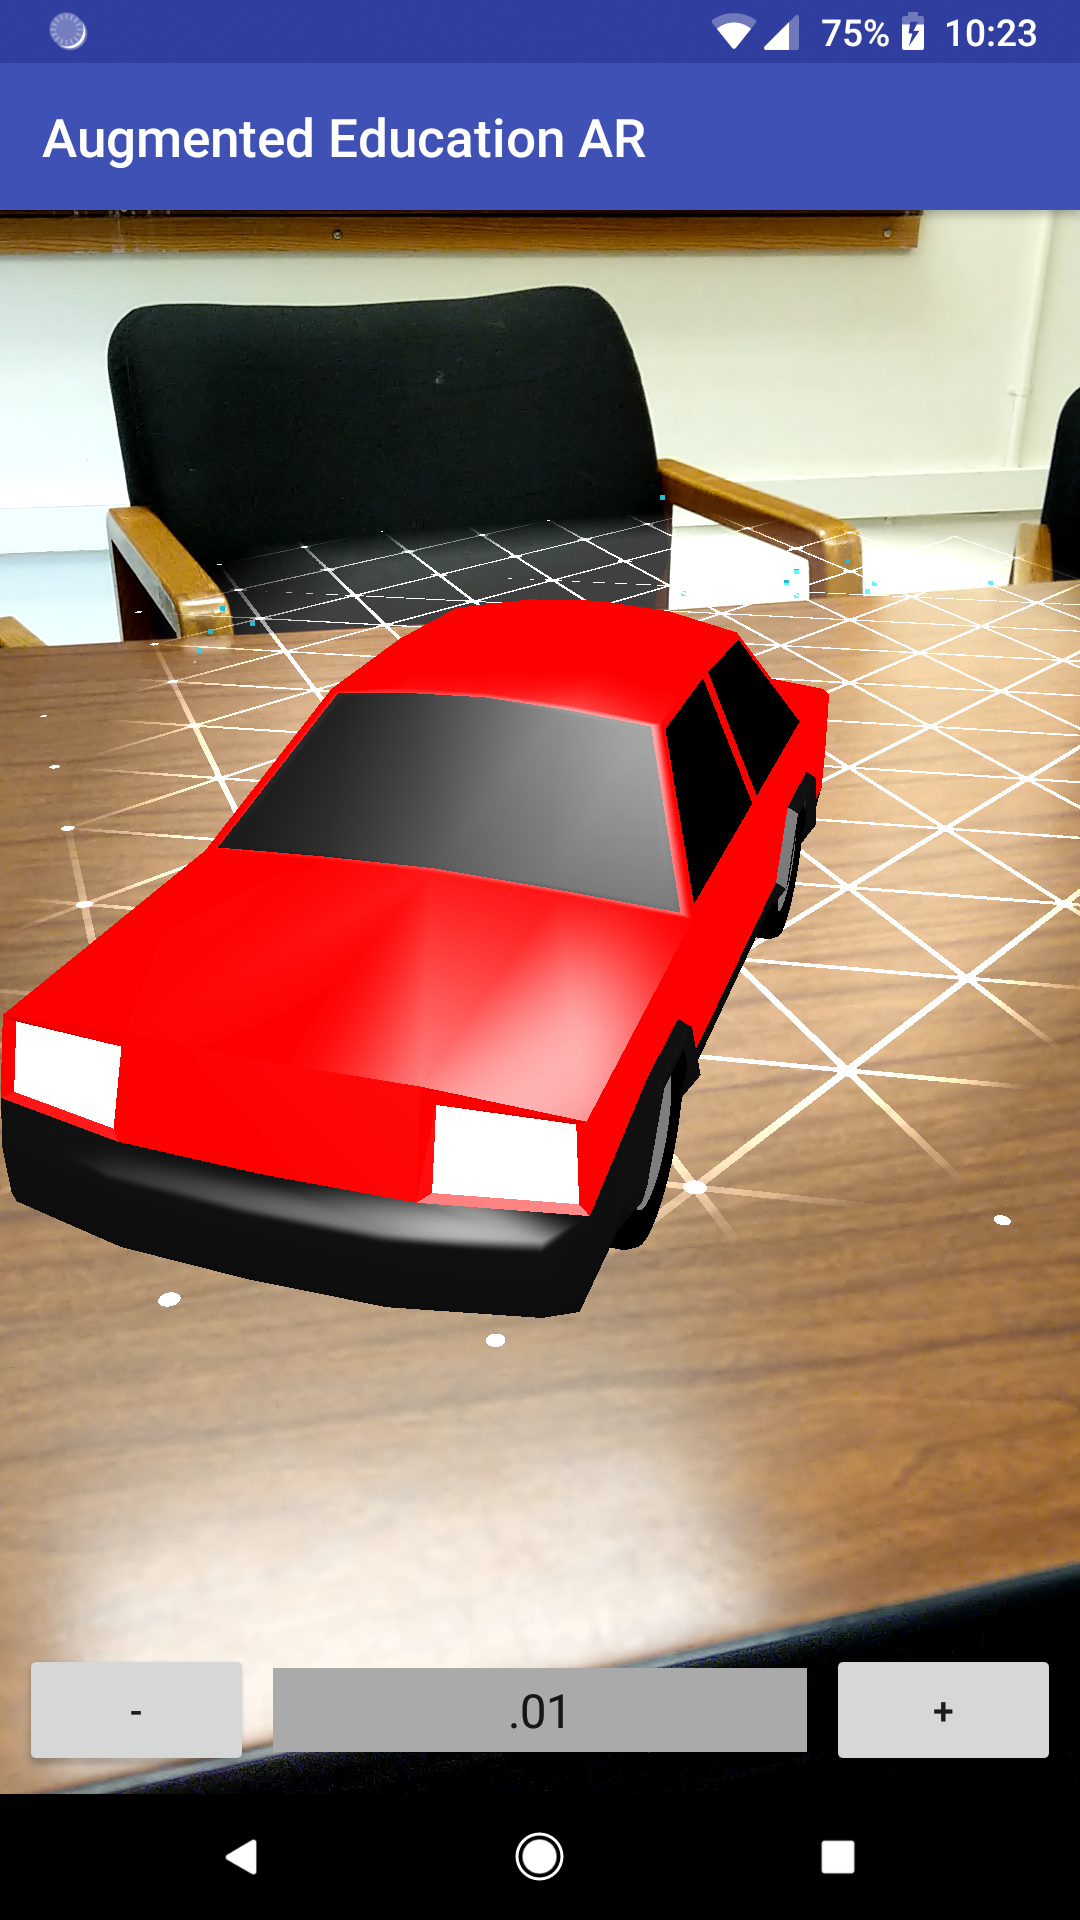
\includegraphics[width=0.5\textwidth]{Mobile/Mobile_Car}
                \centering
                \caption{Colors - Car}
                \label{fig:mobileCar}
            \end{figure}
        
        \subsubsection{Large Files}
        
            One main concern was that 3D files can get large and complex. The BMW is an example of this because it has 51,318 vertices while the sphere has 2258. It took a considerable amount of time to load this file and it draws poorly, showing a limitation of keeping track of so many vertices.
            \begin{figure}[H]
                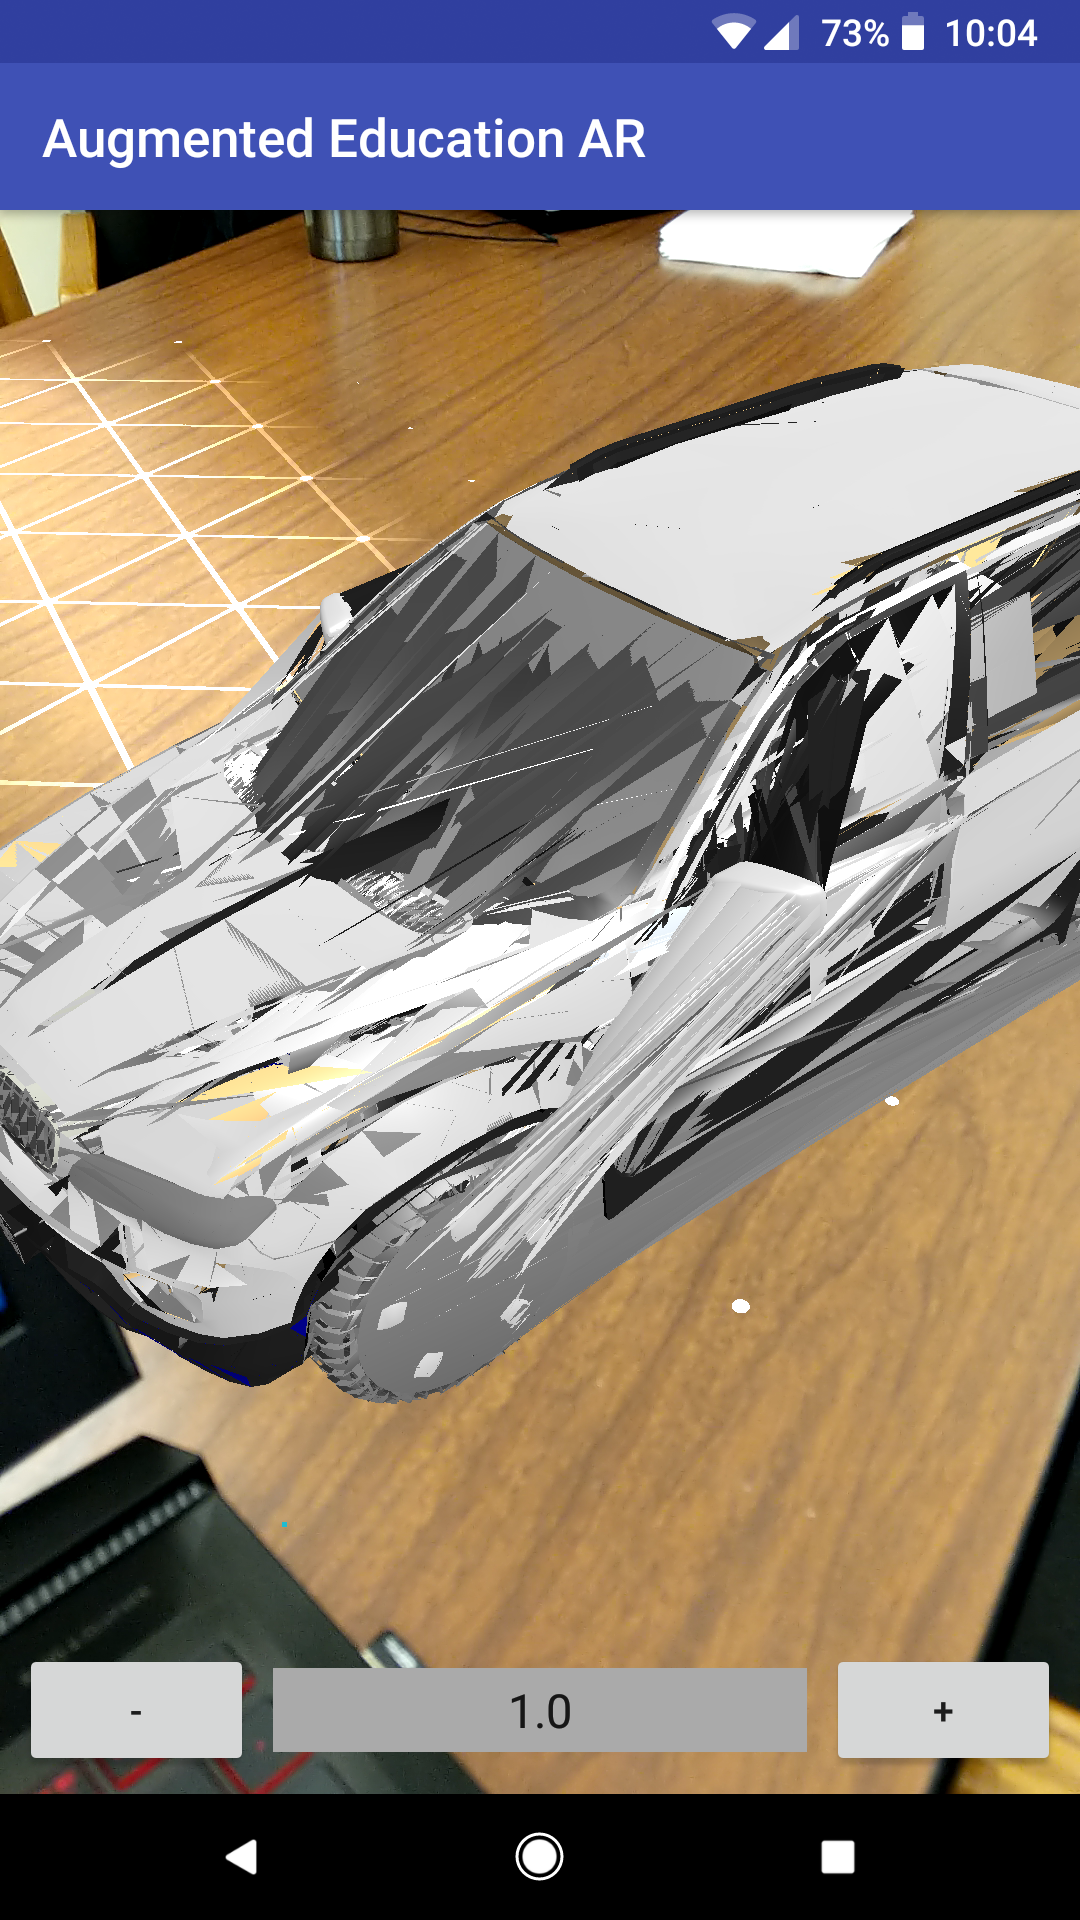
\includegraphics[width=0.5\textwidth]{Mobile/Mobile_BMW}
                \centering
                \caption{Large File - BMW}
                \label{fig:mobileBMW}
            \end{figure}
    
        \subsubsection{Small Files}
            A simple test used especially at the beginning of development to test that models would draw. The sphere is a typical example of something generated from Maple. 
        
            \begin{figure}[H]
                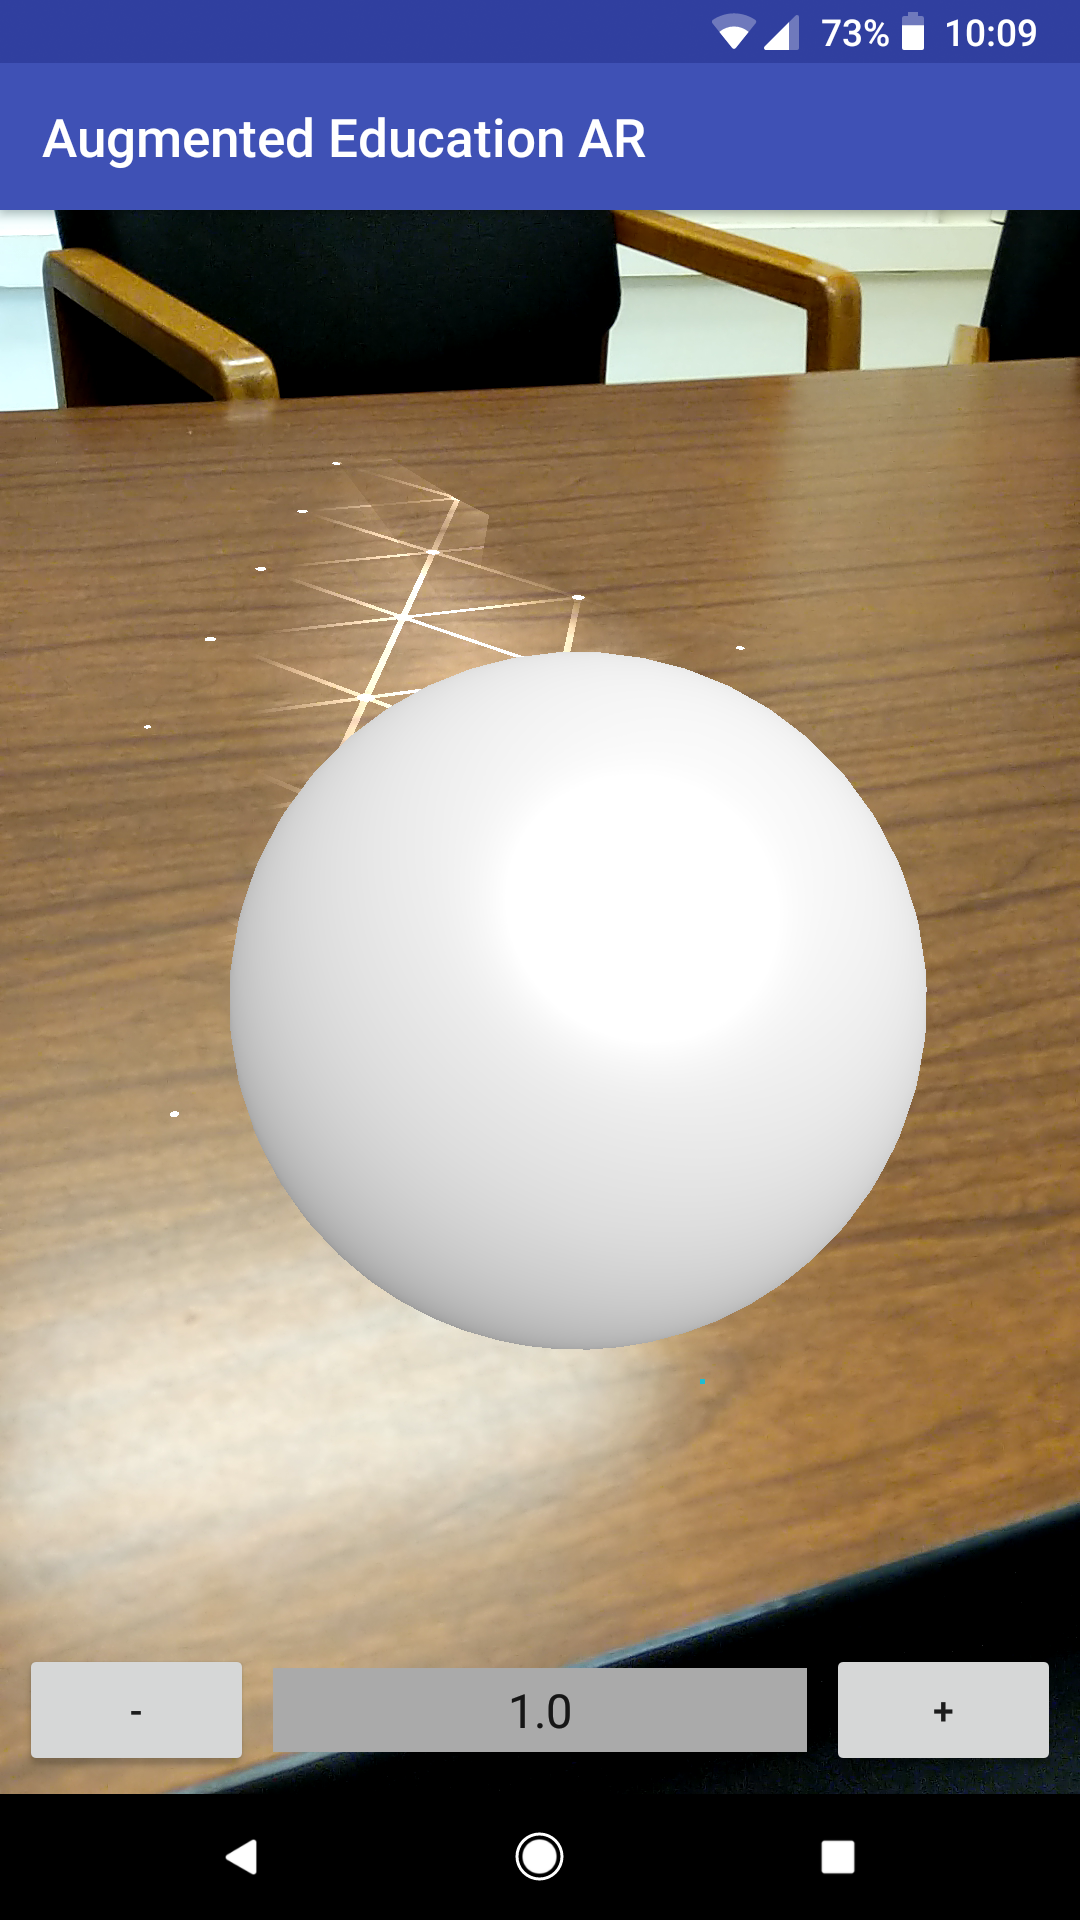
\includegraphics[width=0.5\textwidth]{Mobile/Mobile_Sphere}
                \centering
                \caption{Small File - Sphere}
                \label{fig:mobileSphere}
            \end{figure}
            
        \subsubsection{Embedded Images}
            
            Some 3D modeling software generates OBJ files with PNG textures referenced in the MTL instead of defining RGB values. We needed to test that these files were also supported by our app after adding extra functionality for them. Figure \ref{fig:mobileEmbeddedPhone} shows the PNG texture working, but it doesn't match the intended plot perfectly (Figure \ref{fig:mobileEmbeddedWindows}). This is because the app currently does not support drawing multiple images on top of each other yet.
        
            \begin{figure}[H]
                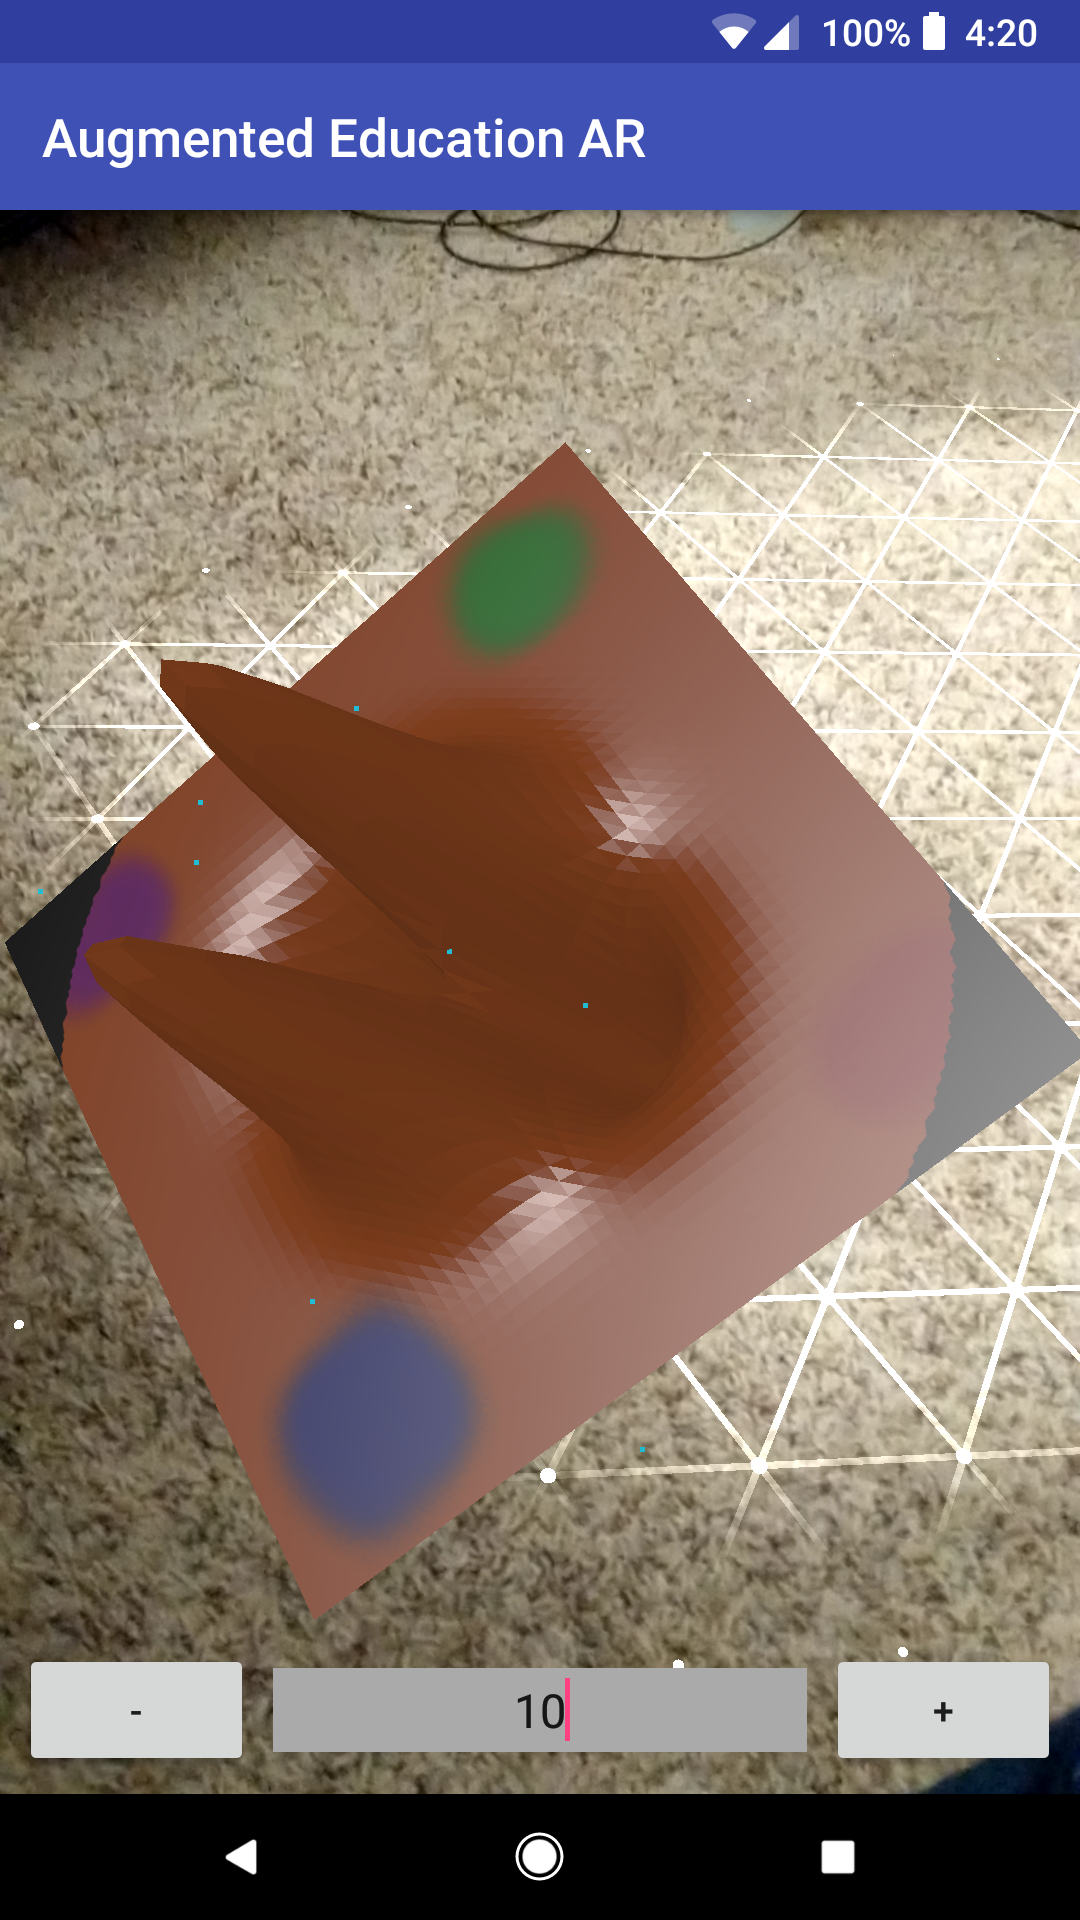
\includegraphics[width=0.5\textwidth]{Mobile/Mobile_ImagesPhone}
                \centering
                \caption{Embedded Image - Viewing on the phone}
                \label{fig:mobileEmbeddedPhone}
            \end{figure}

            \begin{figure}[H]
                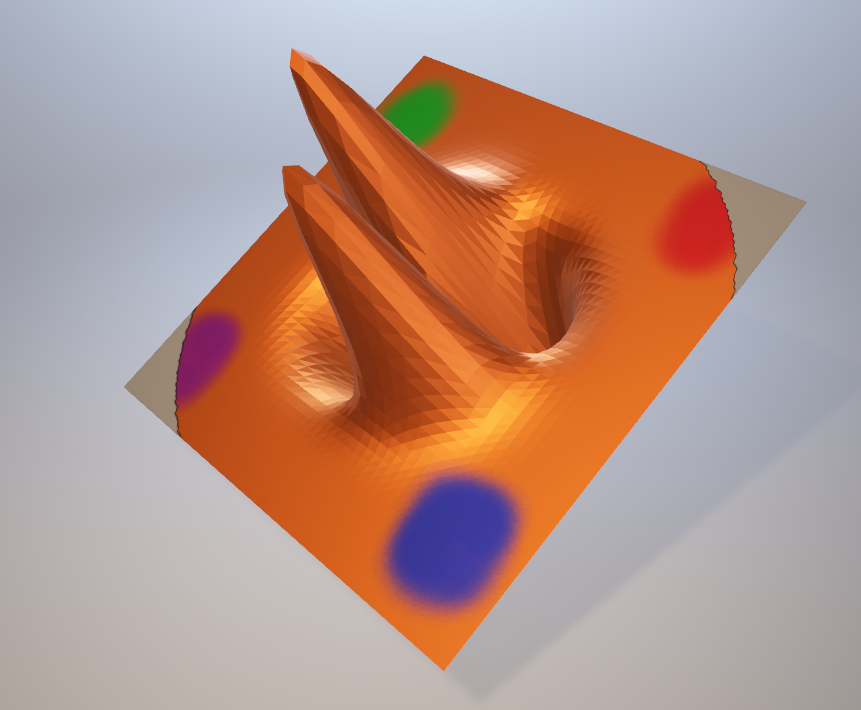
\includegraphics[width=0.5\textwidth]{Mobile/Mobile_ImagesWin}
                \centering
                \caption{Embedded Image - Viewing in the Windows Viewer}
                \label{fig:mobileEmbeddedWindows}
            \end{figure}

        \subsubsection{Scaling}

            Different models scale differently when initially drawn in the app. A scale factor of 1.0 on one model may be too small or too large, making the model difficult to visualize. To remedy this, the app provides an option to increase or decrease the scale factor, as well as change the step so models of different scales can be adjusted properly. Maple models generally need a larger scale factor (approx 3.0) while others like the car need to be adjusted by 0.1 at a time.
        
    \subsection{Web Interface}

        Another major component of the mobile app was the communication with the website.  If the app can display the models, there is little purpose if there is no method to get the models onto the phone.  The web API provided by the web team provides a method for communicating with the website.  It is done using the Volley library, provided by Google.  It abstracts the sending/receiving of networking communication away from the developer.  The code for these interfaces in primarily located in the \texttt{WebAccessor} Java class.

        Testing has shown that while the website is on Azure, the responsiveness is not always the best.  It is not infrequent to receive timeout errors on requests.  When this occurs, a message is displayed to the user.
        
        \subsubsection{Endpoints}
        
            The endpoints used by the mobile application allow the app to: authenticate with the website, get a list of owned models, and download a model.  The endpoints were tested using Postman (to make sure the response was what was expected), the Android Studio debugger to make sure the correct fields were set, and a packet capture application to view the actual HTTP message sent from the phone.

            \paragraph{Authenticate}

                The authentication endpoint allowed the user to provide a username and password to get access to the website.  If the user entered valid credentials, an auth token is returned that allows the application to make requests on behalf of the user.  The auth token is used in the other API calls to the server.

                This API call is only performed on the Main Activity screen (the login page).  If a user is not authenticated, the user cannot continue through the app unless they select the Offline Mode button to not perform future web communication tasks.  A success of this component was, if the user supplied valid credentials, a valid auth token was returned.  Otherwise, an error message should be printed.  The testing was performed manually by trying invalid usernames/passwords.  In these cases, the website did not provide a valid auth token.  When correct usernames/passwords were entered, an auth token is returned.

                The Postman view that was used to test the endpoint (on the web side) is shown in Figure \ref{fig:mobilePostmanGetAuthToken}.

                \begin{figure}[H]
                    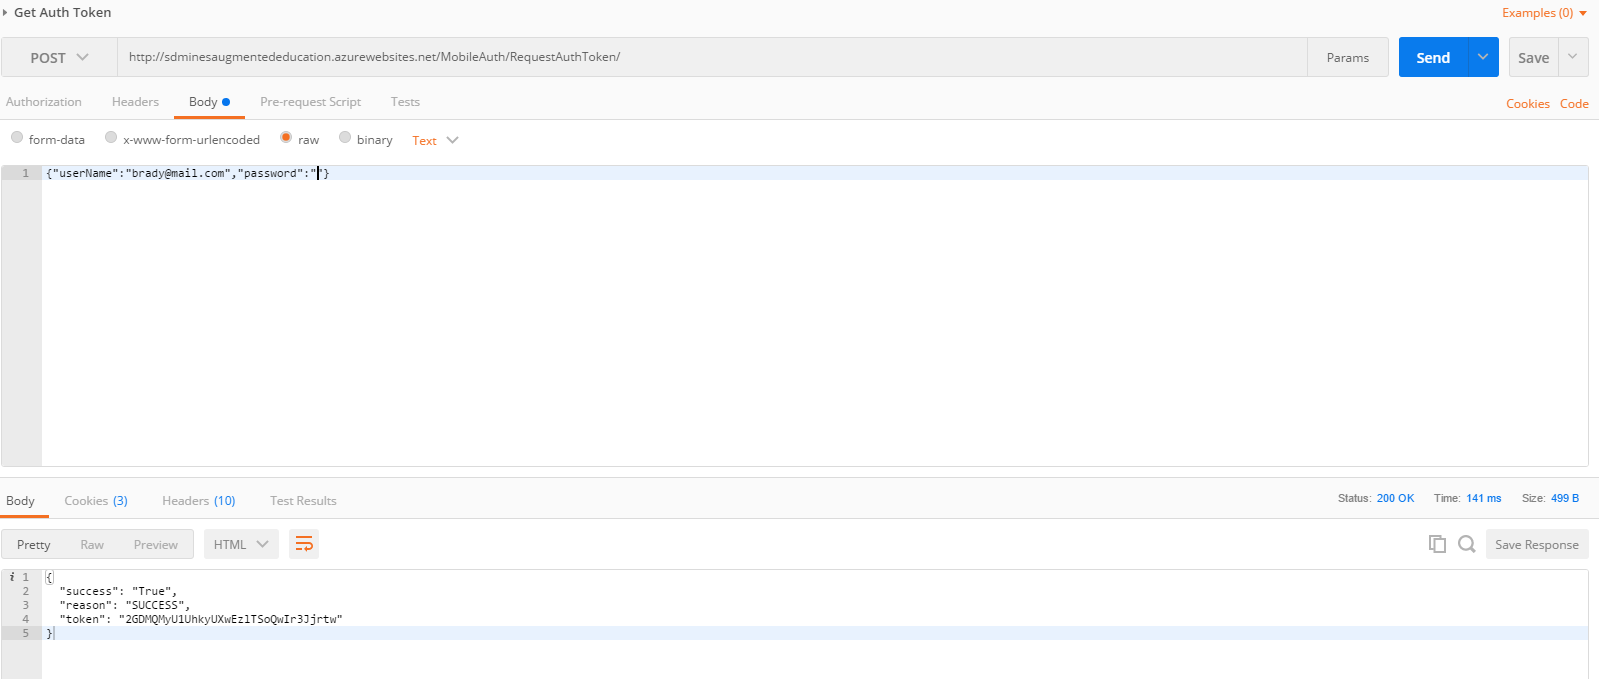
\includegraphics[width=0.75\textwidth]{postman_GetAuthToken}
                    \centering
                    \caption{Postman - Get authentication token}
                    \label{fig:mobilePostmanGetAuthToken}
                \end{figure}
                
            \paragraph{List Models}

                Another endpoint that is used by the mobile device is the one to get a listing of files owned by the user.  Like with the authentication token request, this call was tested manually to ensure the HTTP packets were well formed, and as expected.  Postman was agin used to help test.  Figure \ref{fig:mobilePostmanListFiles} shows the Postman setup to send a request for a file listing.  
                
                \begin{figure}[H]
                    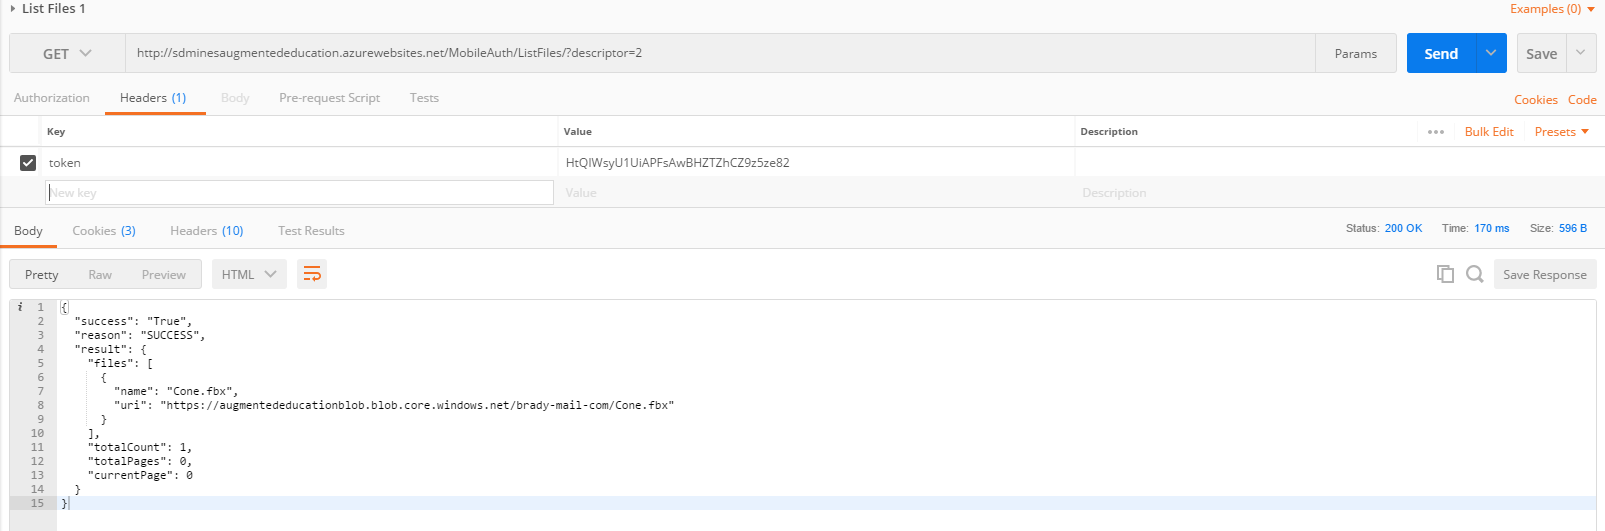
\includegraphics[width=0.75\textwidth]{postman_ListFiles}
                    \centering
                    \caption{Postman - List files}
                    \label{fig:mobilePostmanListFiles}
                \end{figure}
                
                Note, the \texttt{descriptor=} at the end of the url, as it is used to state which files are desired for download.  An agreement was made between the mobile and web teams on what the levels should be.  There is an enumeration defined in the Java code with more details on the values and meanings.  Testing the different values showed a bug in the web code that always caused an error on the mobile device.  This issue was fixed by the web team.
            
            \paragraph{Download Model}

                Downloading a model includes contacting two endpoints.  One is used to get a temporary link to actually download the file, and the next downloads the file from that url.  This is used so the phone can store the long term location, and get a temporary active url to get the file.  Testing for these sections again included using Postman, and using a web browser to facilitate the download.  The Postman settings to get the temporary url are located in Figure \ref{fig:mobilePostmanDownloadFile}.

                \begin{figure}[H]
                    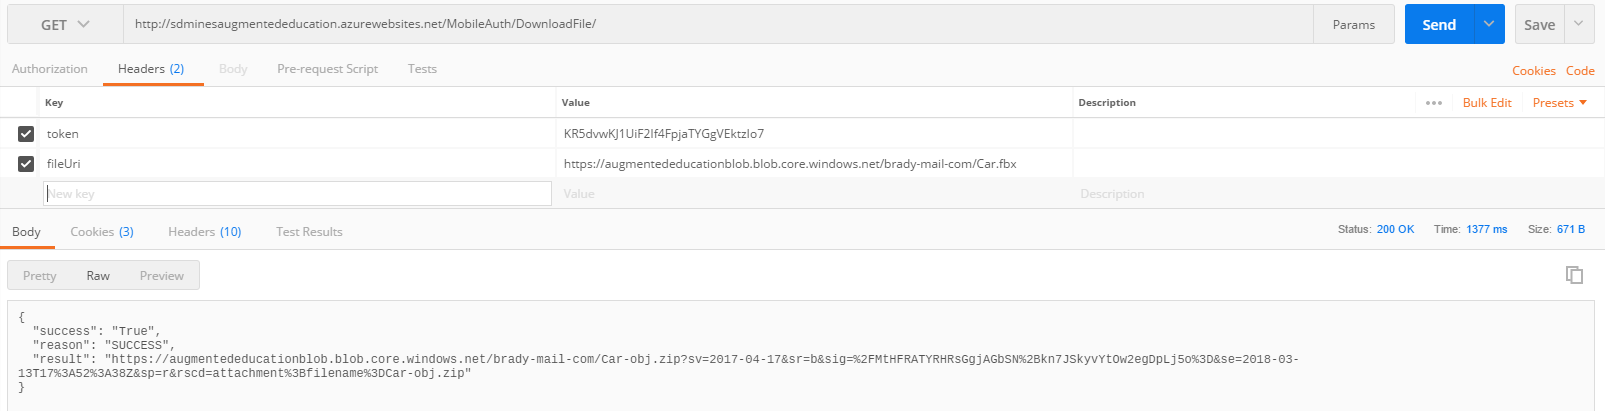
\includegraphics[width=0.75\textwidth]{postman_DownloadFile}
                    \centering
                    \caption{Postman - Download a file}
                    \label{fig:mobilePostmanDownloadFile}
                \end{figure}

                The field \texttt{result} contains the temporary url.  It would then be put into a web browser (typically Firefox or Chrome) and the file is downloaded.  The file downloaded should be in the obj file format, since it is the one that is parse-able by the phone.  The website should use the file conversion software ensure this.  When the models are downloaded, they are stored in a \texttt{Models} directory on the phone.  The file system on the device can be viewed with the Downloads app.  Note, if the model is downloaded, and it does not show up in the file structure, the phone should be restarted.  Commonly, the files do not show up until the device is restarted.  A new folder will be created in the \texttt{Models} directory.  This is because one obj model can have multiple other models associated with it, including mtl (material) files and images.  When the models are downloaded, a zip archive is actually downloaded and extracted.

                Future developers should be aware of how the models are saved from the Android download manager.  When making the call for the download manager to do the download, a final path/file name must be provided.  This can cause issues if the file is saved with the wrong extension, especially if the files are viewed on the developers computer (and not just on the phone).
        
        \subsubsection{No Internet}
        
    \subsection{Offline Mode}

    \subsection{QR Code Scanning}

    \subsection{Database}
